
% Default to the notebook output style

    


% Inherit from the specified cell style.




    
\documentclass{article}

    
    
    \usepackage{graphicx} % Used to insert images
    \usepackage{adjustbox} % Used to constrain images to a maximum size 
    \usepackage{color} % Allow colors to be defined
    \usepackage{enumerate} % Needed for markdown enumerations to work
    \usepackage{geometry} % Used to adjust the document margins
    \usepackage{amsmath} % Equations
    \usepackage{amssymb} % Equations
    \usepackage{eurosym} % defines \euro
    \usepackage[mathletters]{ucs} % Extended unicode (utf-8) support
    \usepackage[utf8x]{inputenc} % Allow utf-8 characters in the tex document
    \usepackage{fancyvrb} % verbatim replacement that allows latex
    \usepackage{grffile} % extends the file name processing of package graphics 
                         % to support a larger range 
    % The hyperref package gives us a pdf with properly built
    % internal navigation ('pdf bookmarks' for the table of contents,
    % internal cross-reference links, web links for URLs, etc.)
    \usepackage{hyperref}
    \usepackage{longtable} % longtable support required by pandoc >1.10
    \usepackage{booktabs}  % table support for pandoc > 1.12.2
    

    
    
    \definecolor{orange}{cmyk}{0,0.4,0.8,0.2}
    \definecolor{darkorange}{rgb}{.71,0.21,0.01}
    \definecolor{darkgreen}{rgb}{.12,.54,.11}
    \definecolor{myteal}{rgb}{.26, .44, .56}
    \definecolor{gray}{gray}{0.45}
    \definecolor{lightgray}{gray}{.95}
    \definecolor{mediumgray}{gray}{.8}
    \definecolor{inputbackground}{rgb}{.95, .95, .85}
    \definecolor{outputbackground}{rgb}{.95, .95, .95}
    \definecolor{traceback}{rgb}{1, .95, .95}
    % ansi colors
    \definecolor{red}{rgb}{.6,0,0}
    \definecolor{green}{rgb}{0,.65,0}
    \definecolor{brown}{rgb}{0.6,0.6,0}
    \definecolor{blue}{rgb}{0,.145,.698}
    \definecolor{purple}{rgb}{.698,.145,.698}
    \definecolor{cyan}{rgb}{0,.698,.698}
    \definecolor{lightgray}{gray}{0.5}
    
    % bright ansi colors
    \definecolor{darkgray}{gray}{0.25}
    \definecolor{lightred}{rgb}{1.0,0.39,0.28}
    \definecolor{lightgreen}{rgb}{0.48,0.99,0.0}
    \definecolor{lightblue}{rgb}{0.53,0.81,0.92}
    \definecolor{lightpurple}{rgb}{0.87,0.63,0.87}
    \definecolor{lightcyan}{rgb}{0.5,1.0,0.83}
    
    % commands and environments needed by pandoc snippets
    % extracted from the output of `pandoc -s`
    \providecommand{\tightlist}{%
      \setlength{\itemsep}{0pt}\setlength{\parskip}{0pt}}
    \DefineVerbatimEnvironment{Highlighting}{Verbatim}{commandchars=\\\{\}}
    % Add ',fontsize=\small' for more characters per line
    \newenvironment{Shaded}{}{}
    \newcommand{\KeywordTok}[1]{\textcolor[rgb]{0.00,0.44,0.13}{\textbf{{#1}}}}
    \newcommand{\DataTypeTok}[1]{\textcolor[rgb]{0.56,0.13,0.00}{{#1}}}
    \newcommand{\DecValTok}[1]{\textcolor[rgb]{0.25,0.63,0.44}{{#1}}}
    \newcommand{\BaseNTok}[1]{\textcolor[rgb]{0.25,0.63,0.44}{{#1}}}
    \newcommand{\FloatTok}[1]{\textcolor[rgb]{0.25,0.63,0.44}{{#1}}}
    \newcommand{\CharTok}[1]{\textcolor[rgb]{0.25,0.44,0.63}{{#1}}}
    \newcommand{\StringTok}[1]{\textcolor[rgb]{0.25,0.44,0.63}{{#1}}}
    \newcommand{\CommentTok}[1]{\textcolor[rgb]{0.38,0.63,0.69}{\textit{{#1}}}}
    \newcommand{\OtherTok}[1]{\textcolor[rgb]{0.00,0.44,0.13}{{#1}}}
    \newcommand{\AlertTok}[1]{\textcolor[rgb]{1.00,0.00,0.00}{\textbf{{#1}}}}
    \newcommand{\FunctionTok}[1]{\textcolor[rgb]{0.02,0.16,0.49}{{#1}}}
    \newcommand{\RegionMarkerTok}[1]{{#1}}
    \newcommand{\ErrorTok}[1]{\textcolor[rgb]{1.00,0.00,0.00}{\textbf{{#1}}}}
    \newcommand{\NormalTok}[1]{{#1}}
    
    \newcommand{\BuiltInTok}[1]{\textcolor[rgb]{0.00,0.44,0.13}{\textbf{{#1}}}}
    \newcommand{\OperatorTok}[1]{\textcolor[rgb]{0.00,0.44,0.13}{\textbf{{#1}}}}
    \newcommand{\ControlFlowTok}[1]{\textcolor[rgb]{0.00,0.44,0.13}{\textbf{{#1}}}}
    \newcommand{\ImportTok}[1]{\textcolor[rgb]{0.00,0.44,0.13}{\textbf{{#1}}}}
    
    % Define a nice break command that doesn't care if a line doesn't already
    % exist.
    \def\br{\hspace*{\fill} \\* }
    % Math Jax compatability definitions
    \def\gt{>}
    \def\lt{<}
    % Document parameters
    \title{02\_01\_1DConvection}
    
    
    

    % Pygments definitions
    
\makeatletter
\def\PY@reset{\let\PY@it=\relax \let\PY@bf=\relax%
    \let\PY@ul=\relax \let\PY@tc=\relax%
    \let\PY@bc=\relax \let\PY@ff=\relax}
\def\PY@tok#1{\csname PY@tok@#1\endcsname}
\def\PY@toks#1+{\ifx\relax#1\empty\else%
    \PY@tok{#1}\expandafter\PY@toks\fi}
\def\PY@do#1{\PY@bc{\PY@tc{\PY@ul{%
    \PY@it{\PY@bf{\PY@ff{#1}}}}}}}
\def\PY#1#2{\PY@reset\PY@toks#1+\relax+\PY@do{#2}}

\expandafter\def\csname PY@tok@kt\endcsname{\def\PY@tc##1{\textcolor[rgb]{0.69,0.00,0.25}{##1}}}
\expandafter\def\csname PY@tok@nc\endcsname{\let\PY@bf=\textbf\def\PY@tc##1{\textcolor[rgb]{0.00,0.00,1.00}{##1}}}
\expandafter\def\csname PY@tok@sd\endcsname{\let\PY@it=\textit\def\PY@tc##1{\textcolor[rgb]{0.73,0.13,0.13}{##1}}}
\expandafter\def\csname PY@tok@vc\endcsname{\def\PY@tc##1{\textcolor[rgb]{0.10,0.09,0.49}{##1}}}
\expandafter\def\csname PY@tok@gi\endcsname{\def\PY@tc##1{\textcolor[rgb]{0.00,0.63,0.00}{##1}}}
\expandafter\def\csname PY@tok@sx\endcsname{\def\PY@tc##1{\textcolor[rgb]{0.00,0.50,0.00}{##1}}}
\expandafter\def\csname PY@tok@ow\endcsname{\let\PY@bf=\textbf\def\PY@tc##1{\textcolor[rgb]{0.67,0.13,1.00}{##1}}}
\expandafter\def\csname PY@tok@bp\endcsname{\def\PY@tc##1{\textcolor[rgb]{0.00,0.50,0.00}{##1}}}
\expandafter\def\csname PY@tok@s1\endcsname{\def\PY@tc##1{\textcolor[rgb]{0.73,0.13,0.13}{##1}}}
\expandafter\def\csname PY@tok@ss\endcsname{\def\PY@tc##1{\textcolor[rgb]{0.10,0.09,0.49}{##1}}}
\expandafter\def\csname PY@tok@vi\endcsname{\def\PY@tc##1{\textcolor[rgb]{0.10,0.09,0.49}{##1}}}
\expandafter\def\csname PY@tok@gu\endcsname{\let\PY@bf=\textbf\def\PY@tc##1{\textcolor[rgb]{0.50,0.00,0.50}{##1}}}
\expandafter\def\csname PY@tok@nv\endcsname{\def\PY@tc##1{\textcolor[rgb]{0.10,0.09,0.49}{##1}}}
\expandafter\def\csname PY@tok@o\endcsname{\def\PY@tc##1{\textcolor[rgb]{0.40,0.40,0.40}{##1}}}
\expandafter\def\csname PY@tok@gp\endcsname{\let\PY@bf=\textbf\def\PY@tc##1{\textcolor[rgb]{0.00,0.00,0.50}{##1}}}
\expandafter\def\csname PY@tok@k\endcsname{\let\PY@bf=\textbf\def\PY@tc##1{\textcolor[rgb]{0.00,0.50,0.00}{##1}}}
\expandafter\def\csname PY@tok@nd\endcsname{\def\PY@tc##1{\textcolor[rgb]{0.67,0.13,1.00}{##1}}}
\expandafter\def\csname PY@tok@vg\endcsname{\def\PY@tc##1{\textcolor[rgb]{0.10,0.09,0.49}{##1}}}
\expandafter\def\csname PY@tok@il\endcsname{\def\PY@tc##1{\textcolor[rgb]{0.40,0.40,0.40}{##1}}}
\expandafter\def\csname PY@tok@cs\endcsname{\let\PY@it=\textit\def\PY@tc##1{\textcolor[rgb]{0.25,0.50,0.50}{##1}}}
\expandafter\def\csname PY@tok@gt\endcsname{\def\PY@tc##1{\textcolor[rgb]{0.00,0.27,0.87}{##1}}}
\expandafter\def\csname PY@tok@mi\endcsname{\def\PY@tc##1{\textcolor[rgb]{0.40,0.40,0.40}{##1}}}
\expandafter\def\csname PY@tok@kr\endcsname{\let\PY@bf=\textbf\def\PY@tc##1{\textcolor[rgb]{0.00,0.50,0.00}{##1}}}
\expandafter\def\csname PY@tok@kc\endcsname{\let\PY@bf=\textbf\def\PY@tc##1{\textcolor[rgb]{0.00,0.50,0.00}{##1}}}
\expandafter\def\csname PY@tok@m\endcsname{\def\PY@tc##1{\textcolor[rgb]{0.40,0.40,0.40}{##1}}}
\expandafter\def\csname PY@tok@ni\endcsname{\let\PY@bf=\textbf\def\PY@tc##1{\textcolor[rgb]{0.60,0.60,0.60}{##1}}}
\expandafter\def\csname PY@tok@mh\endcsname{\def\PY@tc##1{\textcolor[rgb]{0.40,0.40,0.40}{##1}}}
\expandafter\def\csname PY@tok@mb\endcsname{\def\PY@tc##1{\textcolor[rgb]{0.40,0.40,0.40}{##1}}}
\expandafter\def\csname PY@tok@cp\endcsname{\def\PY@tc##1{\textcolor[rgb]{0.74,0.48,0.00}{##1}}}
\expandafter\def\csname PY@tok@na\endcsname{\def\PY@tc##1{\textcolor[rgb]{0.49,0.56,0.16}{##1}}}
\expandafter\def\csname PY@tok@s2\endcsname{\def\PY@tc##1{\textcolor[rgb]{0.73,0.13,0.13}{##1}}}
\expandafter\def\csname PY@tok@nf\endcsname{\def\PY@tc##1{\textcolor[rgb]{0.00,0.00,1.00}{##1}}}
\expandafter\def\csname PY@tok@kd\endcsname{\let\PY@bf=\textbf\def\PY@tc##1{\textcolor[rgb]{0.00,0.50,0.00}{##1}}}
\expandafter\def\csname PY@tok@ge\endcsname{\let\PY@it=\textit}
\expandafter\def\csname PY@tok@nl\endcsname{\def\PY@tc##1{\textcolor[rgb]{0.63,0.63,0.00}{##1}}}
\expandafter\def\csname PY@tok@sr\endcsname{\def\PY@tc##1{\textcolor[rgb]{0.73,0.40,0.53}{##1}}}
\expandafter\def\csname PY@tok@go\endcsname{\def\PY@tc##1{\textcolor[rgb]{0.53,0.53,0.53}{##1}}}
\expandafter\def\csname PY@tok@gh\endcsname{\let\PY@bf=\textbf\def\PY@tc##1{\textcolor[rgb]{0.00,0.00,0.50}{##1}}}
\expandafter\def\csname PY@tok@sb\endcsname{\def\PY@tc##1{\textcolor[rgb]{0.73,0.13,0.13}{##1}}}
\expandafter\def\csname PY@tok@ne\endcsname{\let\PY@bf=\textbf\def\PY@tc##1{\textcolor[rgb]{0.82,0.25,0.23}{##1}}}
\expandafter\def\csname PY@tok@no\endcsname{\def\PY@tc##1{\textcolor[rgb]{0.53,0.00,0.00}{##1}}}
\expandafter\def\csname PY@tok@cm\endcsname{\let\PY@it=\textit\def\PY@tc##1{\textcolor[rgb]{0.25,0.50,0.50}{##1}}}
\expandafter\def\csname PY@tok@w\endcsname{\def\PY@tc##1{\textcolor[rgb]{0.73,0.73,0.73}{##1}}}
\expandafter\def\csname PY@tok@sh\endcsname{\def\PY@tc##1{\textcolor[rgb]{0.73,0.13,0.13}{##1}}}
\expandafter\def\csname PY@tok@gd\endcsname{\def\PY@tc##1{\textcolor[rgb]{0.63,0.00,0.00}{##1}}}
\expandafter\def\csname PY@tok@nn\endcsname{\let\PY@bf=\textbf\def\PY@tc##1{\textcolor[rgb]{0.00,0.00,1.00}{##1}}}
\expandafter\def\csname PY@tok@kp\endcsname{\def\PY@tc##1{\textcolor[rgb]{0.00,0.50,0.00}{##1}}}
\expandafter\def\csname PY@tok@gs\endcsname{\let\PY@bf=\textbf}
\expandafter\def\csname PY@tok@nb\endcsname{\def\PY@tc##1{\textcolor[rgb]{0.00,0.50,0.00}{##1}}}
\expandafter\def\csname PY@tok@gr\endcsname{\def\PY@tc##1{\textcolor[rgb]{1.00,0.00,0.00}{##1}}}
\expandafter\def\csname PY@tok@s\endcsname{\def\PY@tc##1{\textcolor[rgb]{0.73,0.13,0.13}{##1}}}
\expandafter\def\csname PY@tok@c1\endcsname{\let\PY@it=\textit\def\PY@tc##1{\textcolor[rgb]{0.25,0.50,0.50}{##1}}}
\expandafter\def\csname PY@tok@si\endcsname{\let\PY@bf=\textbf\def\PY@tc##1{\textcolor[rgb]{0.73,0.40,0.53}{##1}}}
\expandafter\def\csname PY@tok@se\endcsname{\let\PY@bf=\textbf\def\PY@tc##1{\textcolor[rgb]{0.73,0.40,0.13}{##1}}}
\expandafter\def\csname PY@tok@sc\endcsname{\def\PY@tc##1{\textcolor[rgb]{0.73,0.13,0.13}{##1}}}
\expandafter\def\csname PY@tok@mo\endcsname{\def\PY@tc##1{\textcolor[rgb]{0.40,0.40,0.40}{##1}}}
\expandafter\def\csname PY@tok@c\endcsname{\let\PY@it=\textit\def\PY@tc##1{\textcolor[rgb]{0.25,0.50,0.50}{##1}}}
\expandafter\def\csname PY@tok@err\endcsname{\def\PY@bc##1{\setlength{\fboxsep}{0pt}\fcolorbox[rgb]{1.00,0.00,0.00}{1,1,1}{\strut ##1}}}
\expandafter\def\csname PY@tok@mf\endcsname{\def\PY@tc##1{\textcolor[rgb]{0.40,0.40,0.40}{##1}}}
\expandafter\def\csname PY@tok@nt\endcsname{\let\PY@bf=\textbf\def\PY@tc##1{\textcolor[rgb]{0.00,0.50,0.00}{##1}}}
\expandafter\def\csname PY@tok@kn\endcsname{\let\PY@bf=\textbf\def\PY@tc##1{\textcolor[rgb]{0.00,0.50,0.00}{##1}}}

\def\PYZbs{\char`\\}
\def\PYZus{\char`\_}
\def\PYZob{\char`\{}
\def\PYZcb{\char`\}}
\def\PYZca{\char`\^}
\def\PYZam{\char`\&}
\def\PYZlt{\char`\<}
\def\PYZgt{\char`\>}
\def\PYZsh{\char`\#}
\def\PYZpc{\char`\%}
\def\PYZdl{\char`\$}
\def\PYZhy{\char`\-}
\def\PYZsq{\char`\'}
\def\PYZdq{\char`\"}
\def\PYZti{\char`\~}
% for compatibility with earlier versions
\def\PYZat{@}
\def\PYZlb{[}
\def\PYZrb{]}
\makeatother


    % Exact colors from NB
    \definecolor{incolor}{rgb}{0.0, 0.0, 0.5}
    \definecolor{outcolor}{rgb}{0.545, 0.0, 0.0}



    
    % Prevent overflowing lines due to hard-to-break entities
    \sloppy 
    % Setup hyperref package
    \hypersetup{
      breaklinks=true,  % so long urls are correctly broken across lines
      colorlinks=true,
      urlcolor=blue,
      linkcolor=darkorange,
      citecolor=darkgreen,
      }
    % Slightly bigger margins than the latex defaults
    
    \geometry{verbose,tmargin=1in,bmargin=1in,lmargin=1in,rmargin=1in}
    
    

    \begin{document}
    
    
    \maketitle
    
    

    
    Content under Creative Commons Attribution license CC-BY 4.0, code under
MIT license (c)2014 L.A. Barba, G.F. Forsyth, C.D. Cooper. Based on
\href{https://github.com/barbagroup/CFDPython}{CFD Python}, (c)2013 L.A.
Barba, also under CC-BY.

    \section{Space \& Time}\label{space-time}

    \subsection{Introduction to numerical solution of
PDEs}\label{introduction-to-numerical-solution-of-pdes}

    Welcome to \emph{Space and Time: Introduction to finite-difference
solutions of PDEs}, the second module of
\href{http://openedx.seas.gwu.edu/courses/GW/MAE6286/2014_fall/about}{``Practical
Numerical Methods with Python''}.

In the first module, we looked into numerical integration methods for
the solution of ordinary differential equations (ODEs), using the
phugoid model of glider flight as a motivation. In this module, we will
study the numerical solution of \emph{partial differential equations
(PDEs)}, where the unknown is a multi-variate function. The problem
could depend on time, \(t\), and one spatial dimension \(x\) (or more),
which means we need to build a discretization grid with each independent
variable.

We will start our discussion of numerical PDEs with 1-D linear and
non-linear convection equations, the 1-D diffusion equation, and 1-D
Burgers' equation. We hope you will enjoy them!

    \subsection{1D linear convection}\label{d-linear-convection}

    The \emph{one-dimensional linear convection equation} is the simplest,
most basic model that can be used to learn something about numerical
solution of PDEs. It's surprising that this little equation can teach us
so much! Here it is:

\begin{equation}\frac{\partial u}{\partial t} + c \frac{\partial u}{\partial x} = 0\end{equation}

The equation represents a \emph{wave} propagating with speed \(c\) in
the \(x\) direction, without change of shape. For that reason, it's
sometimes called the \emph{one-way wave equation} (sometimes also the
\emph{advection equation}).

With an initial condition \(u(x,0)=u_0(x)\), the equation has an exact
solution given by:

\begin{equation}u(x,t)=u_0(x-ct). 
\end{equation}

Go on: check it. Take the time and space derivative and stick them into
the equation to see that it holds!

Look at the exact solution for a moment \ldots{} we know two things
about it:

\begin{enumerate}
\def\labelenumi{\arabic{enumi}.}
\tightlist
\item
  its shape does not change, being always the same as the initial wave,
  \(u_0\), only shifted in the \(x\)-direction; and
\item
  it's constant along so-called \textbf{characteristic curves},
  \(x-ct=\)constant. This means that for any point in space and time,
  you can move back along the characteristic curve to \(t=0\) to know
  the value of the solution.
\end{enumerate}

    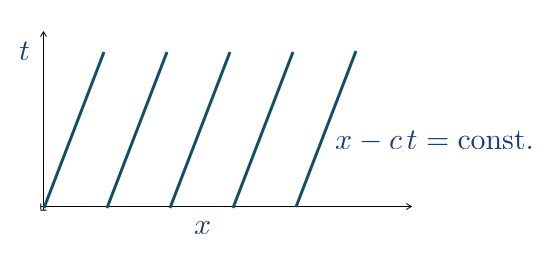
\includegraphics{figures/characteristics.png} \#\#\#\# Characteristic
curves for positive wave speed.

    Why do we call the equations \emph{linear}? PDEs can be either linear or
non-linear. In a linear equation, the unknown function \(u\) and its
derivatives appear only in linear terms, in other words, there are no
products, powers, or transcendental functions applied on them.

What is the most important feature of linear equations? Do you remember?
In case you forgot: solutions can be superposed to generate new
solutions that still satisfy the original equation. This is super
useful!

    \subsection{Finite-differences}\label{finite-differences}

    In the previous lessons, we discretized time derivatives; now we have
derivatives in both space \emph{and} time, so we need to discretize with
respect to \emph{both} these variables.

Imagine a \emph{space-time} plot, where the coordinates in the vertical
direction represent advancing in time---for example, from \(t^n\) to
\(t^{n+1}\)---and the coordinates in the horizontal direction move in
space: consecutive points are \(x_{i-1}\), \(x_i\), and \(x_{i+1}\).
This creates a grid where a point has both a temporal and spatial index.
Here is a graphical representation of the space-time grid:

\textbackslash{}begin\{matrix\} t\^{}\{n+1\} \& $\rightarrow$ \&
$\bullet$  \&\& $\bullet$  \&\& $\bullet$  \textbackslash{} t\^{}n \&
$\rightarrow$ \& $\bullet$  \&\& $\bullet$  \&\& $\bullet$  \textbackslash{} \&
\& x\_\{i-1\} \&\& x\_i \&\& x\_\{i+1\} \textbackslash{}end\{matrix\}

For the numerical solution of \(u(x,t)\), we'll use subscripts to denote
the spatial position, like \(u_i\), and superscripts to denote the
temporal instant, like \(u^n\). We would then label the solution at the
top-middle point in the grid above as follows: \(u^{n+1}_{i}\).

Each grid point below has an index \(i\), corresponding to the spatial
position and increasing to the right, and an index \(n\), corresponding
to the time instant and increasing upwards. A small grid segment would
have the following values of the numerical solution at each point:

\textbackslash{}begin\{matrix\} \& \&$\bullet$ \& \& $\bullet$ \& \&
$\bullet$ \textbackslash{} \& \&u\^{}\{n+1\}\emph{\{i-1\} \& \&
u\^{}\{n+1\}\emph{i \& \& u\^{}\{n+1\}}\{i+1\} \textbackslash{} \&
\&$\bullet$ \& \& $\bullet$ \& \& $\bullet$ \textbackslash{} \&
\&u\^{}n}\{i-1\} \& \& u\^{}n\_i \& \& u\^{}n\_\{i+1\} \textbackslash{}
\& \&$\bullet$ \& \& $\bullet$ \& \& $\bullet$ \textbackslash{} \&
\&u\^{}\{n-1\}\_\{i-1\} \& \& u\^{}\{n-1\}\emph{i \& \&
u\^{}\{n-1\}}\{i+1\} \textbackslash{} \textbackslash{}end\{matrix\}

Another way to explain our discretization grid is to say that it is
built with constant steps in time and space, \(\Delta t\) and
\(\Delta x\), as follows:

\begin{eqnarray}
x_i &=& i\, \Delta x \quad \text{and} \quad t^n= n\, \Delta t \nonumber \\
u_i^n &=& u(i\, \Delta x, n\, \Delta t)
\end{eqnarray}

    \subsubsection{Discretizing our model
equation}\label{discretizing-our-model-equation}

    Let's see how to discretize the 1-D linear convection equation in both
space and time. By definition, the partial derivative with respect to
time changes only with time and not with space; its discretized form
changes only the \(n\) indices. Similarly, the partial derivative with
respect to \(x\) changes with space not time, and only the \(i\) indices
are affected.

We'll discretize the spatial coordinate \(x\) into points indexed from
\(i=0\) to \(N\), and then step in discrete time intervals of size
\(\Delta t\).

From the definition of a derivative (and simply removing the limit), we
know that for \(\Delta x\) sufficiently small:

\begin{equation}\frac{\partial u}{\partial x}\approx \frac{u(x+\Delta x)-u(x)}{\Delta x}\end{equation}

This formula could be applied at any point \(x_i\). But note that it's
not the only way that we can estimate the derivative. The geometrical
interpretation of the first derivative \(\partial u/ \partial x\) at any
point is that it represents the slope of the tangent to the curve
\(u(x)\). In the sketch below, we show a slope line at \(x_i\) and mark
it as ``exact.'' If the formula written above is applied at \(x_i\), it
approximates the derivative using the next spatial grid point: it is
then called a \emph{forward difference} formula.

But as shown in the sketch below, we could also estimate the spatial
derivative using the point behind \(x_i\), in which case it is called a
\emph{backward difference}. We could even use the two points on each
side of \(x_i\), and obtain what's called a \emph{central difference}
(but in that case the denominator would be \(2\Delta x\)).

    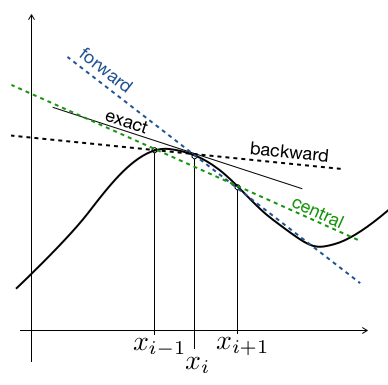
\includegraphics{figures/FDapproxiamtions.png} \#\#\#\# Three
finite-difference approximations at \(x_i\).

    We have three possible ways to represent a discrete form of
\(\partial u/ \partial x\):

\begin{itemize}
\tightlist
\item
  Forward difference: uses \(x_i\) and \(x_i + \Delta x\),
\item
  Backward difference: uses \(x_i\) and \(x_i- \Delta x\),
\item
  Central difference: uses two points on either side of \(x_i\).
\end{itemize}

The sketch above also suggests that some finite-difference formulas
might be better than others: it looks like the \emph{central difference}
approximation is closer to the slope of the ``exact'' derivative.
Curious if this is just an effect of our exaggerated picture? We'll show
you later how to make this observation rigorous!

The three formulas are:

\begin{eqnarray}
\frac{\partial u}{\partial x} & \approx & \frac{u(x_{i+1})-u(x_i)}{\Delta x} \quad\text{Forward}\\
\frac{\partial u}{\partial x} & \approx & \frac{u(x_i)-u(x_{i-1})}{\Delta x} \quad\text{Backward}\\
\frac{\partial u}{\partial x} & \approx & \frac{u(x_{i+1})-u(x_{i-1})}{2\Delta x} \quad\text{Central}
\end{eqnarray}

Euler's method is equivalent to using a forward-difference scheme for
the time derivative. Let's stick with that, and choose the
backward-difference scheme for the space derivative. Our discrete
equation is then:

\begin{equation}\frac{u_i^{n+1}-u_i^n}{\Delta t} + c \frac{u_i^n - u_{i-1}^n}{\Delta x} = 0, \end{equation}

where \(n\) and \(n+1\) are two consecutive steps in time, while \(i-1\)
and \(i\) are two neighboring points of the discretized \(x\)
coordinate. With given initial conditions, the only unknown in this
discretization is \(u_i^{n+1}\). We solve for this unknown to get an
equation that lets us step in time, as follows:

\begin{equation}u_i^{n+1} = u_i^n - c \frac{\Delta t}{\Delta x}(u_i^n-u_{i-1}^n)\end{equation}

We like to make drawings of a grid segment, showing the grid points that
influence our numerical solution. This is called a \textbf{stencil}.
Below is the stencil for solving our model equation with the
finite-difference formula we wrote above.

    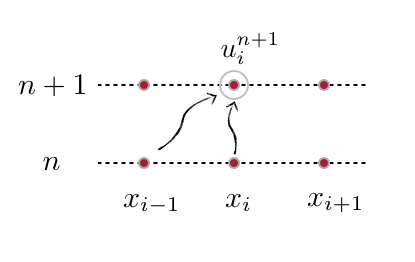
\includegraphics{figures/FTBS_stencil.png} \#\#\#\# Stencil for the
``forward-time/backward-space'' scheme.

    \subsection{And compute!}\label{and-compute}

    Alright. Let's get a little Python on the road. First: we need to load
our array and plotting libraries, as usual. And if you noticed in the
\href{http://nbviewer.ipython.org/github/numerical-mooc/numerical-mooc/blob/master/lessons/01_phugoid/01_04_Second_Order_Methods.ipynb}{\emph{Bonus!}
notebook for Module 1}, we taught you a neat trick to set some global
plotting parameters with the \texttt{rcParams} module. We like to do
that.

    \begin{Verbatim}[commandchars=\\\{\}]
{\color{incolor}In [{\color{incolor}1}]:} \PY{k+kn}{import} \PY{n+nn}{numpy}                       
        \PY{k+kn}{from} \PY{n+nn}{matplotlib} \PY{k}{import} \PY{n}{pyplot}                 
        \PY{o}{\PYZpc{}}\PY{k}{matplotlib} inline
        \PY{k+kn}{from} \PY{n+nn}{matplotlib} \PY{k}{import} \PY{n}{rcParams}
        \PY{n}{rcParams}\PY{p}{[}\PY{l+s}{\PYZsq{}}\PY{l+s}{font.family}\PY{l+s}{\PYZsq{}}\PY{p}{]} \PY{o}{=} \PY{l+s}{\PYZsq{}}\PY{l+s}{serif}\PY{l+s}{\PYZsq{}}
        \PY{n}{rcParams}\PY{p}{[}\PY{l+s}{\PYZsq{}}\PY{l+s}{font.size}\PY{l+s}{\PYZsq{}}\PY{p}{]} \PY{o}{=} \PY{l+m+mi}{16}
\end{Verbatim}

    As a first exercise, we'll solve the 1D linear convection equation with
a \emph{square wave} initial condition, defined as follows:

\begin{equation}
u(x,0)=\begin{cases}2 & \text{where } 0.5\leq x \leq 1,\\
1 & \text{everywhere else in } (0, 2)
\end{cases}
\end{equation}

We also need a boundary condition on \(x\): let \(u=1\) at \(x=0\). Our
spatial domain for the numerical solution will only cover the range
\(x\in (0, 2)\).

    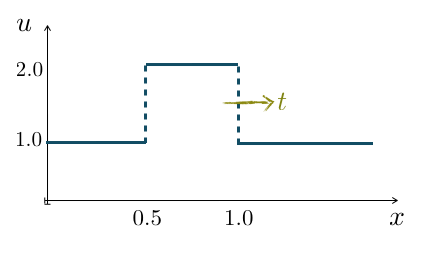
\includegraphics{figures/squarewave.png} \#\#\#\# Square wave initial
condition.

    Now let's define a few variables; we want to make an evenly spaced grid
of points within our spatial domain. In the code below, we define a
variable called \texttt{nx} that will be the number of spatial grid
points, and a variable \texttt{dx} that will be the distance between any
pair of adjacent grid points. We also can define a step in time,
\texttt{dt}, a number of steps, \texttt{nt}, and a value for the wave
speed: we like to keep things simple and make \(c=1\).

    \begin{Verbatim}[commandchars=\\\{\}]
{\color{incolor}In [{\color{incolor}18}]:} \PY{n}{nx} \PY{o}{=} \PY{l+m+mi}{41}  \PY{c}{\PYZsh{} try changing this number from 41 to 81 and Run All ... what happens?}
         \PY{n}{dx} \PY{o}{=} \PY{l+m+mi}{2}\PY{o}{/}\PY{p}{(}\PY{n}{nx}\PY{o}{\PYZhy{}}\PY{l+m+mi}{1}\PY{p}{)}
         \PY{n}{nt} \PY{o}{=} \PY{l+m+mi}{25}    
         \PY{n}{dt} \PY{o}{=} \PY{l+m+mf}{0.04}  
         \PY{n}{c} \PY{o}{=} \PY{l+m+mi}{1}      \PY{c}{\PYZsh{}assume wavespeed of c = 1}
         \PY{n}{x} \PY{o}{=} \PY{n}{numpy}\PY{o}{.}\PY{n}{linspace}\PY{p}{(}\PY{l+m+mi}{0}\PY{p}{,}\PY{l+m+mi}{5}\PY{p}{,}\PY{n}{nx}\PY{p}{)}
         \PY{n+nb}{print} \PY{p}{(}\PY{n}{dx}\PY{p}{)}
\end{Verbatim}

    \begin{Verbatim}[commandchars=\\\{\}]
0.05
    \end{Verbatim}

    We also need to set up our initial conditions. Here, we use the NumPy
function \texttt{ones()} defining an array which is \texttt{nx} elements
long with every value equal to \(1\). How useful! We then \emph{change a
slice} of that array to the value \(u=2\), to get the square wave, and
we print out the initial array just to admire it. But which values
should we change? The problem states that we need to change the indices
of \texttt{u} such that the square wave begins at \(x = 0.5\) and ends
at \(x = 1\).

We can use the \texttt{numpy.where} function to return a list of indices
where the vector \(x\) meets (or doesn't meet) some condition.

    \begin{Verbatim}[commandchars=\\\{\}]
{\color{incolor}In [{\color{incolor}10}]:} \PY{n}{u} \PY{o}{=} \PY{n}{numpy}\PY{o}{.}\PY{n}{ones}\PY{p}{(}\PY{n}{nx}\PY{p}{)}      \PY{c}{\PYZsh{}numpy function ones()}
         \PY{n}{lbound} \PY{o}{=} \PY{n}{numpy}\PY{o}{.}\PY{n}{where}\PY{p}{(}\PY{n}{x} \PY{o}{\PYZgt{}}\PY{o}{=} \PY{l+m+mf}{0.5}\PY{p}{)}
         \PY{n}{ubound} \PY{o}{=} \PY{n}{numpy}\PY{o}{.}\PY{n}{where}\PY{p}{(}\PY{n}{x} \PY{o}{\PYZlt{}}\PY{o}{=} \PY{l+m+mi}{1}\PY{p}{)}
         
         \PY{n+nb}{print}\PY{p}{(}\PY{n}{lbound}\PY{p}{)}
         \PY{n+nb}{print}\PY{p}{(}\PY{n}{ubound}\PY{p}{)}
\end{Verbatim}

    \begin{Verbatim}[commandchars=\\\{\}]
(array([ 4,  5,  6,  7,  8,  9, 10, 11, 12, 13, 14, 15, 16, 17, 18, 19, 20,
       21, 22, 23, 24, 25, 26, 27, 28, 29, 30, 31, 32, 33, 34, 35, 36, 37,
       38, 39, 40], dtype=int64),)
(array([0, 1, 2, 3, 4, 5, 6, 7, 8], dtype=int64),)
    \end{Verbatim}

    That leaves us with two vectors. \texttt{lbound}, which has the indices
for \(x \geq .5\) and `ubound', which has the indices for \(x \leq 1\).
To combine these two, we can use an intersection, with
\texttt{numpy.intersect1d}.

    \begin{Verbatim}[commandchars=\\\{\}]
{\color{incolor}In [{\color{incolor}11}]:} \PY{n}{bounds} \PY{o}{=} \PY{n}{numpy}\PY{o}{.}\PY{n}{intersect1d}\PY{p}{(}\PY{n}{lbound}\PY{p}{,} \PY{n}{ubound}\PY{p}{)}
         \PY{n}{u}\PY{p}{[}\PY{n}{bounds}\PY{p}{]}\PY{o}{=}\PY{l+m+mi}{2}  \PY{c}{\PYZsh{}setting u = 2 between 0.5 and 1 as per our I.C.s}
         \PY{n+nb}{print}\PY{p}{(}\PY{n}{u}\PY{p}{)}
\end{Verbatim}

    \begin{Verbatim}[commandchars=\\\{\}]
[ 1.  1.  1.  1.  2.  2.  2.  2.  2.  1.  1.  1.  1.  1.  1.  1.  1.  1.
  1.  1.  1.  1.  1.  1.  1.  1.  1.  1.  1.  1.  1.  1.  1.  1.  1.  1.
  1.  1.  1.  1.  1.]
    \end{Verbatim}

    Remember that Python can also next commands, we could have instead
written

\begin{Shaded}
  \begin{Highlighting}[]
    \NormalTok{u[numpy.intersect1d(numpy.where(x }\OperatorTok{>=} \FloatTok{0.5}\NormalTok{), numpy.where(x }\OperatorTok{<=} \DecValTok{1}\NormalTok{))] }\OperatorTok{=} \DecValTok{2}
  \end{Highlighting}
\end{Shaded}

but that can be a little hard to read.

    Now let's take a look at those initial conditions we've built with a
handy plot.

    \begin{Verbatim}[commandchars=\\\{\}]
{\color{incolor}In [{\color{incolor}12}]:} \PY{n}{pyplot}\PY{o}{.}\PY{n}{plot}\PY{p}{(}\PY{n}{x}\PY{p}{,} \PY{n}{u}\PY{p}{,} \PY{n}{color}\PY{o}{=}\PY{l+s}{\PYZsq{}}\PY{l+s}{\PYZsh{}003366}\PY{l+s}{\PYZsq{}}\PY{p}{,} \PY{n}{ls}\PY{o}{=}\PY{l+s}{\PYZsq{}}\PY{l+s}{\PYZhy{}\PYZhy{}}\PY{l+s}{\PYZsq{}}\PY{p}{,} \PY{n}{lw}\PY{o}{=}\PY{l+m+mi}{2}\PY{p}{)}
         \PY{n}{pyplot}\PY{o}{.}\PY{n}{ylim}\PY{p}{(}\PY{l+m+mi}{0}\PY{p}{,}\PY{l+m+mf}{2.5}\PY{p}{)}\PY{p}{;}
\end{Verbatim}

    \begin{center}
    \adjustimage{max size={0.9\linewidth}{0.9\paperheight}}{02_01_1DConvection_files/02_01_1DConvection_28_0.png}
    \end{center}
    { \hspace*{\fill} \\}
    
    It does look pretty close to what we expected. But it looks like the
sides of the square wave are not perfectly vertical. Is that right?
Think for a bit.

    Now it's time to write some code for the discrete form of the convection
equation using our chosen finite-difference scheme.

For every element of our array \texttt{u}, we need to perform the
operation:

\[u_i^{n+1} = u_i^n - c \frac{\Delta t}{\Delta x}(u_i^n-u_{i-1}^n)\]

We'll store the result in a new (temporary) array \texttt{un}, which
will be the solution \(u\) for the next time-step. We will repeat this
operation for as many time-steps as we specify and then we can see how
far the wave has traveled.

We first initialize the placeholder array \texttt{un} to hold the values
we calculate for the \(n+1\) timestep, using once again the NumPy
function \texttt{ones()}.

Then, we may think we have two iterative operations: one in space and
one in time (we'll learn differently later), so we may start by nesting
a spatial loop inside the time loop, as shown below. You see that the
code for the finite-difference scheme is a direct expression of the
discrete equation:

    \begin{Verbatim}[commandchars=\\\{\}]
{\color{incolor}In [{\color{incolor}26}]:} \PY{k}{for} \PY{n}{n} \PY{o+ow}{in} \PY{n+nb}{range}\PY{p}{(}\PY{l+m+mi}{1}\PY{p}{,}\PY{n}{nt}\PY{p}{)}\PY{p}{:}  
             \PY{n}{un} \PY{o}{=} \PY{n}{u}\PY{o}{.}\PY{n}{copy}\PY{p}{(}\PY{p}{)} 
             \PY{k}{for} \PY{n}{i} \PY{o+ow}{in} \PY{n+nb}{range}\PY{p}{(}\PY{l+m+mi}{1}\PY{p}{,}\PY{n}{nx}\PY{p}{)}\PY{p}{:} 
                 \PY{n}{u}\PY{p}{[}\PY{n}{i}\PY{p}{]} \PY{o}{=} \PY{n}{un}\PY{p}{[}\PY{n}{i}\PY{p}{]}\PY{o}{\PYZhy{}}\PY{n}{c}\PY{o}{*}\PY{n}{dt}\PY{o}{/}\PY{n}{dx}\PY{o}{*}\PY{p}{(}\PY{n}{un}\PY{p}{[}\PY{n}{i}\PY{p}{]}\PY{o}{\PYZhy{}}\PY{n}{un}\PY{p}{[}\PY{n}{i}\PY{o}{\PYZhy{}}\PY{l+m+mi}{1}\PY{p}{]}\PY{p}{)}
\end{Verbatim}

    \textbf{Note}---We will learn later that the code as written above is
quite inefficient, and there are better ways to write this,
Python-style. But let's carry on.

Now let's inspect our solution array after advancing in time with a line
plot.

    \begin{Verbatim}[commandchars=\\\{\}]
{\color{incolor}In [{\color{incolor}25}]:} \PY{n}{pyplot}\PY{o}{.}\PY{n}{plot}\PY{p}{(}\PY{n}{x}\PY{p}{,} \PY{n}{u}\PY{p}{,} \PY{n}{color}\PY{o}{=}\PY{l+s}{\PYZsq{}}\PY{l+s}{\PYZsh{}003366}\PY{l+s}{\PYZsq{}}\PY{p}{,} \PY{n}{ls}\PY{o}{=}\PY{l+s}{\PYZsq{}}\PY{l+s}{\PYZhy{}\PYZhy{}}\PY{l+s}{\PYZsq{}}\PY{p}{,} \PY{n}{lw}\PY{o}{=}\PY{l+m+mi}{3}\PY{p}{)}
         \PY{n}{pyplot}\PY{o}{.}\PY{n}{ylim}\PY{p}{(}\PY{l+m+mi}{0}\PY{p}{,}\PY{l+m+mf}{2.5}\PY{p}{)}\PY{p}{;}
\end{Verbatim}

    \begin{center}
    \adjustimage{max size={0.9\linewidth}{0.9\paperheight}}{02_01_1DConvection_files/02_01_1DConvection_33_0.png}
    \end{center}
    { \hspace*{\fill} \\}
    
    That's funny. Our square wave has definitely moved to the right, but
it's no longer in the shape of a top-hat. \textbf{What's going on?}

    \subparagraph{Dig deeper}\label{dig-deeper}

    The solution differs from the expected square wave because the
discretized equation is an approximation of the continuous differential
equation that we want to solve. There are errors: we knew that. But the
modified shape of the initial wave is something curious. Maybe it can be
improved by making the grid spacing finer. Why don't you try it? Does it
help?

    \subsection{Spatial truncation error}\label{spatial-truncation-error}

    Recall the finite-difference approximation we are using for the spatial
derivative:

\begin{equation}\frac{\partial u}{\partial x}\approx \frac{u(x+\Delta x)-u(x)}{\Delta x}\end{equation}

We obtain it by using the definition of the derivative at a point, and
simply removing the limit, in the assumption that \(\Delta x\) is very
small. But we already learned with Euler's method that this introduces
an error, called the \emph{truncation error}.

Using a Taylor series expansion for the spatial terms now, we see that
the backward-difference scheme produces a first-order method, in space.

    \begin{equation}
\frac{\partial u}{\partial x}(x_i) = \frac{u(x_i)-u(x_{i-1})}{\Delta x} + \frac{\Delta x}{2} \frac{\partial^2 u}{\partial x^2}(x_i) - \frac{\Delta x^2}{6} \frac{\partial^3 u}{\partial x^3}(x_i)+ \cdots
\end{equation}

The dominant term that is neglected in the finite-difference
approximation is of \(\mathcal{O}(\Delta x)\). We also see that the
approximation \emph{converges} to the exact derivative as
\(\Delta x \rightarrow 0\). That's good news!

In summary, the chosen ``forward-time/backward space'' difference scheme
is first-order in both space and time: the truncation errors are
\(\mathcal{O}(\Delta t, \Delta x)\). We'll come back to this!

    \subsection{Non-linear convection}\label{non-linear-convection}

    Let's move on to the non-linear convection equation, using the same
methods as before. The 1-D convection equation is:

\begin{equation}\frac{\partial u}{\partial t} + u \frac{\partial u}{\partial x} = 0\end{equation}

The only difference with the linear case is that we've replaced the
constant wave speed \(c\) by the variable speed \(u\). The equation is
non-linear because now we have a product of the solution and one of its
derivatives: the product \(u\,\partial u/\partial x\). This changes
everything!

We're going to use the same discretization as for linear convection:
forward difference in time and backward difference in space. Here is the
discretized equation:

\begin{equation}\frac{u_i^{n+1}-u_i^n}{\Delta t} + u_i^n \frac{u_i^n-u_{i-1}^n}{\Delta x} = 0\end{equation}

Solving for the only unknown term, \(u_i^{n+1}\), gives an equation that
can be used to advance in time:

\begin{equation}u_i^{n+1} = u_i^n - u_i^n \frac{\Delta t}{\Delta x} (u_i^n - u_{i-1}^n)\end{equation}

There is very little that needs to change from the code written so far.
In fact, we'll even use the same square-wave initial condition. But
let's re-initialize the variable \texttt{u} with the initial values, and
re-enter the numerical parameters here, for convenience (we no longer
need \(c\), though).

    \begin{Verbatim}[commandchars=\\\{\}]
{\color{incolor}In [{\color{incolor}126}]:} \PY{c}{\PYZsh{}\PYZsh{}problem parameters}
          \PY{n}{nx} \PY{o}{=} \PY{l+m+mi}{41}
          \PY{n}{dx} \PY{o}{=} \PY{l+m+mi}{2}\PY{o}{/}\PY{p}{(}\PY{n}{nx}\PY{o}{\PYZhy{}}\PY{l+m+mi}{1}\PY{p}{)}
          \PY{n}{nt} \PY{o}{=} \PY{l+m+mi}{10}    
          \PY{n}{dt} \PY{o}{=} \PY{o}{.}\PY{l+m+mi}{02}  
          
          \PY{c}{\PYZsh{}\PYZsh{}initial conditions}
          \PY{n}{u} \PY{o}{=} \PY{n}{numpy}\PY{o}{.}\PY{n}{ones}\PY{p}{(}\PY{n}{nx}\PY{p}{)}      
          \PY{n}{u}\PY{p}{[}\PY{n}{numpy}\PY{o}{.}\PY{n}{intersect1d}\PY{p}{(}\PY{n}{lbound}\PY{p}{,} \PY{n}{ubound}\PY{p}{)}\PY{p}{]}\PY{o}{=}\PY{l+m+mi}{2}  
          \PY{n+nb}{print} \PY{p}{(}\PY{n}{x}\PY{p}{)}
          \PY{n+nb}{print} \PY{p}{(}\PY{n}{u}\PY{p}{)}
\end{Verbatim}

    \begin{Verbatim}[commandchars=\\\{\}]
[ 0.    0.05  0.1   0.15  0.2   0.25  0.3   0.35  0.4   0.45  0.5   0.55
  0.6   0.65  0.7   0.75  0.8   0.85  0.9   0.95  1.    1.05  1.1   1.15
  1.2   1.25  1.3   1.35  1.4   1.45  1.5   1.55  1.6   1.65  1.7   1.75
  1.8   1.85  1.9   1.95  2.  ]
[ 1.  1.  1.  1.  1.  1.  1.  1.  1.  1.  2.  2.  2.  2.  2.  2.  2.  2.
  2.  2.  2.  1.  1.  1.  1.  1.  1.  1.  1.  1.  1.  1.  1.  1.  1.  1.
  1.  1.  1.  1.  1.]
    \end{Verbatim}

    How does it look?

    \begin{Verbatim}[commandchars=\\\{\}]
{\color{incolor}In [{\color{incolor}127}]:} \PY{n}{pyplot}\PY{o}{.}\PY{n}{plot}\PY{p}{(}\PY{n}{x}\PY{p}{,} \PY{n}{u}\PY{p}{,} \PY{n}{color}\PY{o}{=}\PY{l+s}{\PYZsq{}}\PY{l+s}{\PYZsh{}003366}\PY{l+s}{\PYZsq{}}\PY{p}{,} \PY{n}{ls}\PY{o}{=}\PY{l+s}{\PYZsq{}}\PY{l+s}{\PYZhy{}\PYZhy{}}\PY{l+s}{\PYZsq{}}\PY{p}{,} \PY{n}{lw}\PY{o}{=}\PY{l+m+mi}{3}\PY{p}{)}
          \PY{n}{pyplot}\PY{o}{.}\PY{n}{ylim}\PY{p}{(}\PY{l+m+mi}{0}\PY{p}{,}\PY{l+m+mf}{2.5}\PY{p}{)}\PY{p}{;}
\end{Verbatim}

    \begin{center}
    \adjustimage{max size={0.9\linewidth}{0.9\paperheight}}{02_01_1DConvection_files/02_01_1DConvection_44_0.png}
    \end{center}
    { \hspace*{\fill} \\}
    
    Changing just one line of code in the solution of linear convection, we
are able to now get the non-linear solution: the line that corresponds
to the discrete equation now has \texttt{un{[}i{]}} in the place where
before we just had \texttt{c}. So you could write something like:

\begin{Shaded}
\begin{Highlighting}[]
\ControlFlowTok{for} \NormalTok{n }\OperatorTok{in} \BuiltInTok{range}\NormalTok{(}\DecValTok{1}\NormalTok{,nt):  }
  \NormalTok{un }\OperatorTok{=} \NormalTok{u.copy() }
  \ControlFlowTok{for} \NormalTok{i }\OperatorTok{in} \BuiltInTok{range}\NormalTok{(}\DecValTok{1}\NormalTok{,nx): }
    \NormalTok{u[i] }\OperatorTok{=} \NormalTok{un[i]}\OperatorTok{-}\NormalTok{un[i]}\OperatorTok{*}\NormalTok{dt}\OperatorTok{/}\NormalTok{dx}\OperatorTok{*}\NormalTok{(un[i]}\OperatorTok{-}\NormalTok{un[i}\DecValTok{-1}\NormalTok{]) }
\end{Highlighting}
\end{Shaded}

We're going to be more clever than that and use NumPy to update all
values of the spatial grid in one fell swoop. We don't really need to
write a line of code that gets executed \emph{for each} value of \(u\)
on the spatial grid. Python can update them all at once! Study the code
below, and compare it with the one above. Here is a helpful sketch, to
illustrate the array operation---also called a ``vectorized''
operation---for \(u_i-u_{i-1}\).

    \begin{figure}[htbp]
\centering
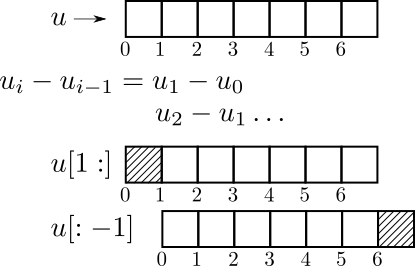
\includegraphics{figures/vectorizedstencil.png}
\caption{vectorizedstencil}
\end{figure}

 \#\#\#\# Sketch to explain vectorized stencil operation. Adapted from
\href{https://blog.nelhage.com/2015/08/indices-point-between-elements/}{``Indices
point between elements''} by Nelson Elhage.

    \begin{Verbatim}[commandchars=\\\{\}]
{\color{incolor}In [{\color{incolor}128}]:} \PY{k}{for} \PY{n}{n} \PY{o+ow}{in} \PY{n+nb}{range}\PY{p}{(}\PY{l+m+mi}{1}\PY{p}{,} \PY{n}{nt}\PY{p}{)}\PY{p}{:}  
              \PY{n}{un} \PY{o}{=} \PY{n}{u}\PY{o}{.}\PY{n}{copy}\PY{p}{(}\PY{p}{)} 
              \PY{n}{u}\PY{p}{[}\PY{l+m+mi}{1}\PY{p}{:}\PY{p}{]} \PY{o}{=} \PY{n}{un}\PY{p}{[}\PY{l+m+mi}{1}\PY{p}{:}\PY{p}{]}\PY{o}{\PYZhy{}}\PY{n}{un}\PY{p}{[}\PY{l+m+mi}{1}\PY{p}{:}\PY{p}{]}\PY{o}{*}\PY{n}{dt}\PY{o}{/}\PY{n}{dx}\PY{o}{*}\PY{p}{(}\PY{n}{un}\PY{p}{[}\PY{l+m+mi}{1}\PY{p}{:}\PY{p}{]}\PY{o}{\PYZhy{}}\PY{n}{un}\PY{p}{[}\PY{l+m+mi}{0}\PY{p}{:}\PY{o}{\PYZhy{}}\PY{l+m+mi}{1}\PY{p}{]}\PY{p}{)} 
              \PY{n}{u}\PY{p}{[}\PY{l+m+mi}{0}\PY{p}{]} \PY{o}{=} \PY{l+m+mf}{1.0}
\end{Verbatim}

    \begin{Verbatim}[commandchars=\\\{\}]
{\color{incolor}In [{\color{incolor}129}]:} \PY{n}{pyplot}\PY{o}{.}\PY{n}{plot}\PY{p}{(}\PY{n}{x}\PY{p}{,} \PY{n}{u}\PY{p}{,} \PY{n}{color}\PY{o}{=}\PY{l+s}{\PYZsq{}}\PY{l+s}{\PYZsh{}003366}\PY{l+s}{\PYZsq{}}\PY{p}{,} \PY{n}{ls}\PY{o}{=}\PY{l+s}{\PYZsq{}}\PY{l+s}{\PYZhy{}\PYZhy{}}\PY{l+s}{\PYZsq{}}\PY{p}{,} \PY{n}{lw}\PY{o}{=}\PY{l+m+mi}{3}\PY{p}{)}
          \PY{n}{pyplot}\PY{o}{.}\PY{n}{ylim}\PY{p}{(}\PY{l+m+mi}{0}\PY{p}{,}\PY{l+m+mf}{2.5}\PY{p}{)}\PY{p}{;}
\end{Verbatim}

    \begin{center}
    \adjustimage{max size={0.9\linewidth}{0.9\paperheight}}{02_01_1DConvection_files/02_01_1DConvection_48_0.png}
    \end{center}
    { \hspace*{\fill} \\}
    
    Hmm. That's quite interesting: like in the linear case, we see that we
have lost the sharp sides of our initial square wave, but there's more.
Now, the wave has also lost symmetry! It seems to be lagging on the rear
side, while the front of the wave is steepening. Is this another form of
numerical error, do you ask? No! It's physics!

    \subparagraph{Dig deeper}\label{dig-deeper}

    Think about the effect of having replaced the constant wave speed \(c\)
by the variable speed given by the solution \(u\). It means that
different parts of the wave move at different speeds. Make a sketch of
an initial wave and think about where the speed is higher and where it
is lower \ldots{}

    \subsection{References}\label{references}

\begin{itemize}
\tightlist
\item
  Elhage, Nelson (2015),
  \href{https://blog.nelhage.com/2015/08/indices-point-between-elements/}{``Indices
  point between elements''}
\end{itemize}

    \begin{center}\rule{0.5\linewidth}{\linethickness}\end{center}

The cell below loads the style of the notebook.

    \begin{Verbatim}[commandchars=\\\{\}]
{\color{incolor}In [{\color{incolor}1}]:} \PY{k+kn}{from} \PY{n+nn}{IPython}\PY{n+nn}{.}\PY{n+nn}{core}\PY{n+nn}{.}\PY{n+nn}{display} \PY{k}{import} \PY{n}{HTML}
        \PY{n}{css\PYZus{}file} \PY{o}{=} \PY{l+s}{\PYZsq{}}\PY{l+s}{../../styles/numericalmoocstyle.css}\PY{l+s}{\PYZsq{}}
        \PY{n}{HTML}\PY{p}{(}\PY{n+nb}{open}\PY{p}{(}\PY{n}{css\PYZus{}file}\PY{p}{,} \PY{l+s}{\PYZdq{}}\PY{l+s}{r}\PY{l+s}{\PYZdq{}}\PY{p}{)}\PY{o}{.}\PY{n}{read}\PY{p}{(}\PY{p}{)}\PY{p}{)}
\end{Verbatim}

            \begin{Verbatim}[commandchars=\\\{\}]
{\color{outcolor}Out[{\color{outcolor}1}]:} <IPython.core.display.HTML object>
\end{Verbatim}
        
    \begin{Verbatim}[commandchars=\\\{\}]
{\color{incolor}In [{\color{incolor} }]:} 
\end{Verbatim}


    % Add a bibliography block to the postdoc
    
    
    
    \end{document}
